\documentclass[aspectratio=169,10pt]{beamer}
\usetheme{metropolis}
\usepackage{amsmath,amssymb,bm}
\usepackage{siunitx}
\usepackage{booktabs}
\usepackage[table]{xcolor}
\usepackage{tikz}
\usetikzlibrary{arrows.meta,calc,positioning,patterns}
\usepackage{pgfplots}
\pgfplotsset{compat=1.17}
\sisetup{per-mode=symbol,detect-all}
\metroset{numbering=fraction,progressbar=frametitle,block=fill}
\tikzset{capt/.style={text width=5.2cm,align=center}}
\hypersetup{colorlinks=true,urlcolor=blue!60!black,linkcolor=.}
\addtobeamertemplate{frametitle}{}{%
  \begin{tikzpicture}[remember picture,overlay]
    \node[anchor=north east,yshift=-1.5pt,xshift=-6pt] at (current page.north east) {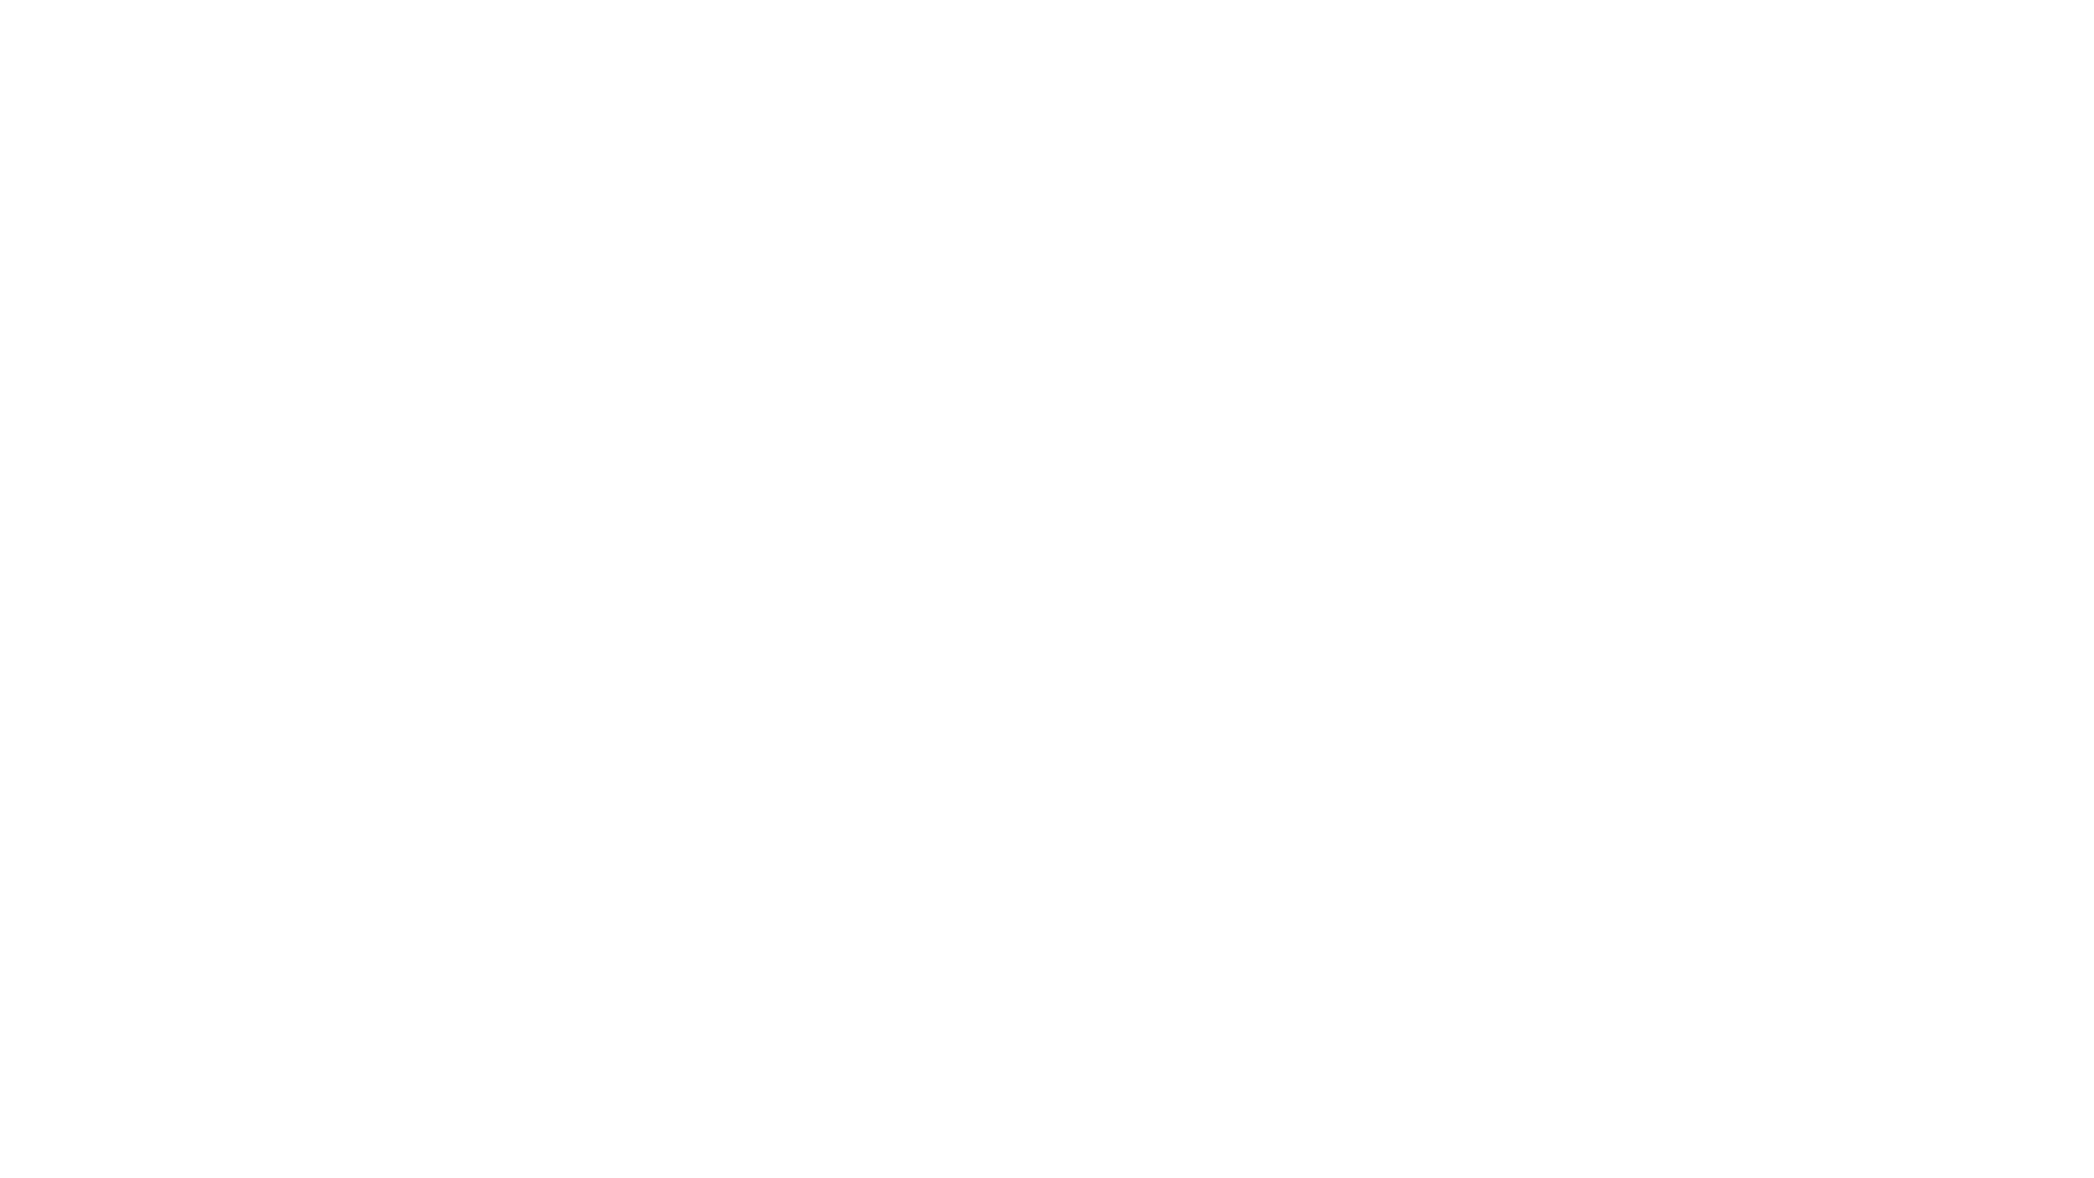
\includegraphics[height=0.7cm]{logos/itu_logo_beyaz.pdf}};
  \end{tikzpicture}}
\titlegraphic{\hfill
\includegraphics[height=1.6cm]{logos/itu_logo_laci.pdf}}

\title{Lecture 6: Tension and Shear Joints}
\subtitle{UCK 364E Design of Machine Elements}
\author{Prof.\ Dr.\ Onur Tunçer}
\institute{Department of Aeronautical Engineering, Istanbul Technical University}
\date{Fall 2026}


\begin{document}
\maketitle

\begin{frame}{Today}
\begin{enumerate}
  \item Two kinds of joint --- and why they share nothing but hardware
  \item The joint diagram, and how an external load divides
  \item Yielding, separation, and the cliff between them
  \item Fatigue of the preloaded bolt --- and what preload is really for
  \item Shear joints: four failure modes, four margins
  \item Edge distance and pitch --- what they are actually protecting
  \item Why fasteners in a row do not share the load
  \item Rivets --- and the types still flying
  \item Eccentric bolt groups
  \item Combined tension and shear --- and why the grip decides the exponent
\end{enumerate}
\end{frame}

\section{Two kinds of joint}

\begin{frame}{Lecture 5 gave you the fastener. This gives you the joint.}
A bolt that is perfectly specified --- right thread, right class, right preload --- will still fail
if the joint around it was analysed in the \alert{wrong direction}.
\vfill
\centering\footnotesize
\begin{tabular}{@{}lll@{}}
\toprule
 & \textbf{Tension joint} & \textbf{Shear joint}\\
\midrule
The load is & along the bolt axis & across it\\
What carries it & the \emph{clamp}, until it separates & bolt in shear, plate in bearing\\
Preload is & the whole design variable & not a strength you may count on\\
You check & yield, separation, fatigue & bolt shear, bearing, net tension, shear-out\\
Usually governs & fatigue & bearing, or the plate\\
It fails by & the bolt stretching, the joint opening & the hole elongating, the plate tearing\\
\bottomrule
\end{tabular}
\vfill
\raggedright
And one thing in common: a \textbf{fitting factor of 1.15} on every joint, fitting and bearing
surface, on top of the 1.5 (CS/FAR 25.625).
\end{frame}

\begin{frame}{Why preload is not a shear strength}
\begin{columns}[T]
\begin{column}{0.48\textwidth}
\begin{block}{In tension}
The preload \textbf{is} the design. The bolt never sees the external load directly --- only $C$ of
it --- for as long as the joint stays shut.
\end{block}
\end{column}
\begin{column}{0.48\textwidth}
\begin{alertblock}{In shear}
Preload stops fretting and keeps the joint rigid. It is \textbf{not} a certifiable load path:
friction depends on a coefficient nobody can guarantee.
\vspace{2pt}
So the bolt bears against the hole, and you size it for bearing.
\end{alertblock}
\end{column}
\end{columns}
\end{frame}

\section{The preloaded joint under tension}

\begin{frame}{Everything follows from one picture}
\centering
\resizebox{!}{5.5cm}{% The joint diagram. Numbers are the M10 joint of Lecture 5: ki=485, km=1936 kN/mm, Fi=36.1 kN, P=20 kN.
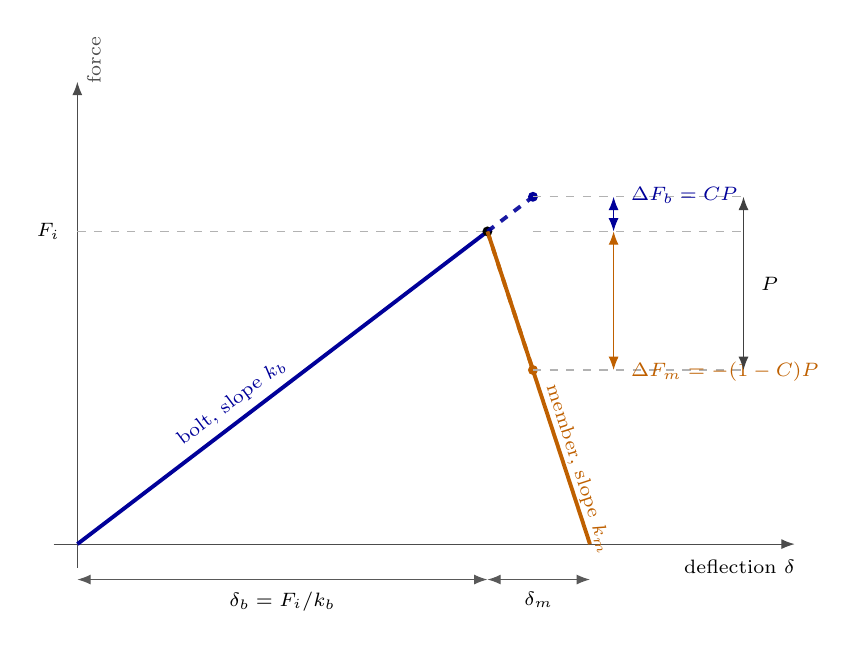
\begin{tikzpicture}[>=Latex,line join=round]
\tikzset{
  bolt/.style={blue!60!black,line width=1.4pt},
  memb/.style={orange!75!black,line width=1.4pt},
  thin2/.style={gray!60,thin},
  dimn/.style={<->,gray!70!black,thin},
  lb/.style={font=\scriptsize},
  key/.style={font=\scriptsize,align=left}
}
\def\xs{70}      % mm  -> cm
\def\ys{0.11}    % kN  -> cm
\pgfmathsetmacro\db{0.0744*\xs}     % bolt stretch at preload
\pgfmathsetmacro\dm{0.0186*\xs}     % member squash at preload
\pgfmathsetmacro\Fi{36.1*\ys}
\pgfmathsetmacro\dd{0.00826*\xs}    % extra deflection under P
\pgfmathsetmacro\Fb{40.1*\ys}
\pgfmathsetmacro\Fm{20.1*\ys}
\pgfmathsetmacro\base{\db+\dm}
\pgfmathsetmacro\Fmid{(\Fb+\Fm)/2}

% axes
\draw[->,black!70] (-0.3,0) -- (\base+2.6,0);
\node[font=\scriptsize,anchor=north] at (\base+1.9,-0.08) {deflection $\delta$};
\draw[->,black!70] (0,-0.3) -- (0,\Fi+1.9) node[anchor=north west,font=\scriptsize,rotate=90,xshift=-4pt] {force};

% ---- the two springs at preload ----
\draw[bolt] (0,0) -- (\db,\Fi);
\draw[memb] (\base,0) -- (\db,\Fi);
\node[lb,text=blue!60!black,anchor=south east,rotate=37] at (\db*0.55,\Fi*0.55) {bolt, slope $k_b$};
\node[lb,text=orange!75!black,anchor=south west,rotate=-72] at (\db+\dm*0.42,\Fi*0.52) {member, slope $k_m$};

% preload level
\draw[thin2,dashed] (0,\Fi) -- (\db,\Fi);
\node[lb,anchor=east] at (-0.1,\Fi) {$F_i$};
\fill[black] (\db,\Fi) circle (1.8pt);

% ---- after the external load P is applied ----
\draw[bolt,dashed,opacity=0.9] (\db,\Fi) -- (\db+\dd,\Fb);
\draw[memb,dashed,opacity=0.9] (\db,\Fi) -- (\db+\dd,\Fm);
\fill[blue!60!black] (\db+\dd,\Fb) circle (1.8pt);
\fill[orange!75!black] (\db+\dd,\Fm) circle (1.8pt);

% the split of P
\draw[thin2,dashed] (\db+\dd,\Fb) -- (\base+1.95,\Fb);
\draw[thin2,dashed] (\db+\dd,\Fm) -- (\base+1.95,\Fm);
\draw[thin2,dashed] (\db+\dd,\Fi) -- (\base+1.95,\Fi);

\draw[dimn,blue!60!black] (\base+0.30,\Fi) -- (\base+0.30,\Fb);
\node[lb,text=blue!60!black,anchor=west] at (\base+0.40,\Fb+0.02) {$\Delta F_b = CP$};
\draw[dimn,orange!75!black] (\base+0.30,\Fm) -- (\base+0.30,\Fi);
\node[lb,text=orange!75!black,anchor=west] at (\base+0.40,\Fm-0.02) {$\Delta F_m = -(1-C)P$};
\draw[dimn,black!75] (\base+1.95,\Fm) -- (\base+1.95,\Fb);
\node[lb,anchor=west] at (\base+2.05,\Fmid) {$P$};

% deflections at preload
\draw[dimn] (0,-0.45) -- (\db,-0.45);
\node[lb,anchor=north] at (\db/2,-0.48) {$\delta_b = F_i/k_b$};
\draw[dimn] (\db,-0.45) -- (\base,-0.45);
\node[lb,anchor=north] at (\db+\dm/2,-0.48) {$\delta_m$};

\end{tikzpicture}
}
\vfill
\raggedright
Bolt and members must deflect \textbf{together}. That is what splits the external load.
\end{frame}

\begin{frame}{How the load divides}
\[
F_b = F_i + C\,P
\qquad\qquad
F_m = F_i - (1-C)\,P
\qquad\qquad
C=\frac{k_b}{k_b+k_m}
\]
\vfill
\begin{alertblock}{Look at the signs}
The \textbf{bolt load barely rises}. The \textbf{clamp force falls fast}.
\vspace{2pt}
For the M10 joint of Lecture 5 with $C=0.20$: a \SI{20}{kN} external load adds \SI{4}{kN} to the
bolt --- and removes \SI{16}{kN} of clamp.
\end{alertblock}
\vfill
\centering
That asymmetry is the whole subject.
\end{frame}

\begin{frame}{Two things can go wrong --- and they pull opposite ways}
\begin{columns}[T]
\begin{column}{0.48\textwidth}
\begin{block}{Yielding}
\[ \sigma_b=\frac{F_i+CP}{A_t}\le S_p \]
\[ n_p=\frac{S_pA_t-F_i}{C\,P} \]
\vspace{-4pt}
Raise the preload and this margin \alert{falls}.
\end{block}
\end{column}
\begin{column}{0.48\textwidth}
\begin{block}{Separation}
\[ F_m=0 \ \Rightarrow\ P_0=\frac{F_i}{1-C} \]
\[ n_0=\frac{F_i}{P\,(1-C)} \]
\vspace{-4pt}
Raise the preload and this margin \alert{rises}.
\end{block}
\end{column}
\end{columns}
\vfill
\centering
The preload is squeezed from both sides. That is why $F_i$ is a \textbf{decision}, not a default.
\end{frame}

\begin{frame}{Separation is not a serviceability issue. It is a cliff.}
\begin{alertblock}{A joint that has separated is a different machine}
The members no longer share the load, so the bolt carries \textbf{all} of $P$ instead of $CP$.
\vspace{3pt}
An instant multiplication by $1/C$ --- typically \textbf{four to eight times}.
\vspace{3pt}
Everything you calculated about fatigue is void from that moment.
\end{alertblock}
\vfill
\centering
\large We will put a number on this in two slides.
\end{frame}

\section{Fatigue of the preloaded joint}

\begin{frame}{The calculation Lecture 5 kept deferring}
External load fluctuating $0 \to P$. The bolt sees only $C$ of it:
\[
\sigma_a=\frac{C\,P}{2A_t},\qquad \sigma_i=\frac{F_i}{A_t},\qquad \sigma_m=\sigma_a+\sigma_i
\]
\vfill
The load line starts at $(\sigma_i,0)$ and rises at \textbf{45\textdegree} --- every increment of
alternating stress brings an equal increment of mean stress. Intersect with Goodman:
\[
\frac{\sigma_a}{S_e}+\frac{\sigma_i+\sigma_a}{S_{ut}}=1
\quad\Longrightarrow\quad
\sigma_{a,\text{lim}}=\frac{S_e(S_{ut}-\sigma_i)}{S_{ut}+S_e}
\]
\vfill
\centering
\[
n_f=\frac{S_e\,(S_{ut}-\sigma_i)}{\sigma_a\,(S_{ut}+S_e)}
\]
\end{frame}

\begin{frame}{The thing everyone gets backwards}
\begin{center}\Large
$\sigma_a = \dfrac{CP}{2A_t}$ \qquad \alert{contains no $F_i$}
\end{center}
\vfill
Once the joint is closed, \textbf{increasing the preload does not reduce the alternating stress}.
It only raises the mean stress --- which by Goodman makes $n_f$ slightly \emph{worse}.
\vfill
\begin{alertblock}{So why preload hard?}
Because of the cliff. Preload's job is to \textbf{guarantee the joint never opens}, and the
alternating stress is small only while that is true.
\vspace{2pt}
Preload does not reduce the fatigue load. It protects the condition under which the fatigue load is
small. \emph{Only the second statement is true.}
\end{alertblock}
\vfill
\centering
What \emph{does} reduce $\sigma_a$ is reducing $C$: a longer, more slender bolt; stiffer members; a washer.
\end{frame}

\begin{frame}{Example 6.1 --- the M10 joint, now with an external load}
M10$\times$1.5 class 10.9. $A_t=\SI{58}{mm^2}$, $S_p=\SI{830}{MPa}$, $S_{ut}=\SI{1040}{MPa}$,
$S_e=\SI{162}{MPa}$. \ $k_b=485$, $k_m=\SI{1936}{kN/mm} \Rightarrow C=0.200$.
\ $F_i=0.75F_p=\SI{36.1}{kN}$. \ External load $0\to P=\SI{20}{kN}$.
\vfill
\begin{columns}[T]
\begin{column}{0.47\textwidth}
\begin{block}{Static}
$F_b = 36.1+0.2(20)=\SI{40.1}{kN}$
\vspace{2pt}
$n_p=\dfrac{48.1-36.1}{4.0}=\mathbf{3.00}$
\vspace{2pt}
$n_0=\dfrac{36.1}{20(0.8)}=\mathbf{2.26}$
\end{block}
\end{column}
\begin{column}{0.49\textwidth}
\begin{block}{Fatigue}
$\sigma_a=\SI{34.5}{MPa}$, \ $\sigma_i=\SI{622}{MPa}$
\vspace{2pt}
$n_f=\dfrac{162(1040-622)}{34.5(1202)}=\mathbf{1.63}$
\vspace{2pt}
\alert{Fatigue governs.}
\end{block}
\end{column}
\end{columns}
\end{frame}

\begin{frame}{Now the cliff, with numbers}
Suppose the joint separates --- preload lost, or $P$ exceeded $P_0=\SI{45.1}{kN}$. The bolt now
carries \emph{all} of $P$:
\[
\sigma_a=\frac{20\,000}{2(58)}=\SI{172}{MPa}
\qquad\text{exactly } 1/C = 5\times \text{ the closed-joint value}
\]
\vfill
With $\sigma_m=\sigma_a$, Goodman gives
\[
n=\left(\frac{172}{162}+\frac{172}{1040}\right)^{-1}=\alert{\mathbf{0.81}}
\]
\vfill
\begin{alertblock}{}
\centering\large
The joint with a comfortable fatigue margin of \textbf{1.63} fails in fatigue\\ the moment it opens.
\vspace{2pt}
\normalsize That is what the preload buys --- and it is the only thing it buys.
\end{alertblock}
\end{frame}

\begin{frame}{Choosing the preload}
Run Example 6.1 again at three preloads:
\vfill
\centering\small
\begin{tabular}{@{}lccc@{}}
\toprule
Preload & $n_p$ (yield) & $n_0$ (separation) & $n_f$ (fatigue)\\
\midrule
$0.90F_p$ & 1.20 & 2.71 & 1.14\\
$\mathbf{0.75F_p}$ & \textbf{3.00} & \textbf{2.26} & \textbf{1.63}\\
$0.50F_p$ & 6.01 & 1.50 & 2.44\\
\bottomrule
\end{tabular}
\vfill
\raggedright
Two of three margins \emph{improve} as preload falls. Taken at face value that argues for a low
preload --- and it is wrong, because $n_0$ guards the cliff, \alert{and the preload you set is not
the preload you get}: $\pm\SI{25}{\percent}$ with a torque wrench.
\vfill
\centering
A nominal $0.5F_p$ can arrive at $0.37F_p$, and $n_0$ falls to 1.1.
\end{frame}

\begin{frame}{Hence the rule --- and now you know why}
\begin{center}
\Large
$F_i = 0.75\,F_p$ \ (reused joints) \qquad $F_i = 0.90\,F_p$ \ (permanent joints)
\end{center}
\vfill
\begin{columns}[T]
\begin{column}{0.48\textwidth}
\begin{block}{High enough}
that the \textbf{worst} end of the scatter still cannot open the joint.
\end{block}
\end{column}
\begin{column}{0.48\textwidth}
\begin{block}{Low enough}
that the \textbf{best} end of the scatter still cannot yield the bolt.
\end{block}
\end{column}
\end{columns}
\vfill
\centering
It is a scatter-management rule, not a strength rule.
\end{frame}

\section{Shear joints}

\begin{frame}{Turn the load through ninety degrees}
\centering
\resizebox{0.98\textwidth}{!}{% The four ways a shear joint fails. Panel 1 in elevation, panels 2-4 in plan.
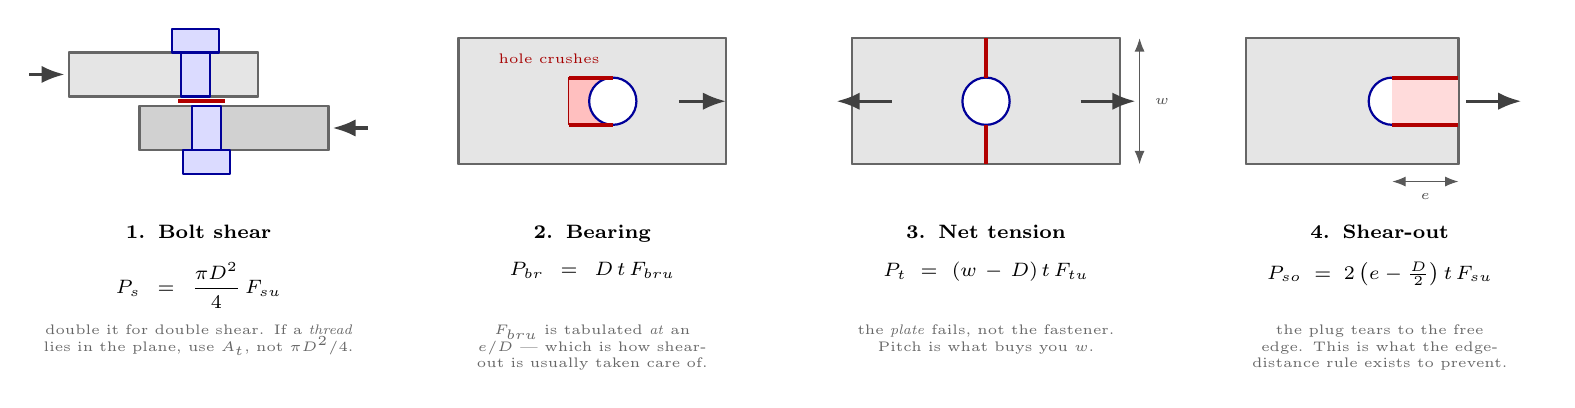
\begin{tikzpicture}[>=Latex,line join=round]
\tikzset{
  plate/.style={fill=black!10,draw=black!60,thick},
  plate2/.style={fill=black!18,draw=black!60,thick},
  blt/.style={fill=blue!14,draw=blue!60!black,thick},
  fail/.style={red!70!black,line width=1.5pt},
  crush/.style={fill=red!25,draw=red!65!black,thin},
  ld/.style={->,black!75,line width=1.2pt},
  ttl/.style={font=\scriptsize\bfseries,align=center,text width=3.9cm,anchor=north},
  frm/.style={font=\scriptsize,align=center,text width=4.0cm,anchor=north},
  sub/.style={font=\tiny,align=center,text width=4.0cm,text=black!60,anchor=north},
  dimn/.style={<->,gray!70!black,thin}
}

%================= 1. bolt shear (elevation) =================
\def\x{0}
\fill[plate]  (\x-1.65,0.06) rectangle (\x+0.75,0.62);
\fill[plate2] (\x-0.75,-0.62) rectangle (\x+1.65,-0.06);
\draw[black!60,thick] (\x-1.65,0.06) rectangle (\x+0.75,0.62);
\draw[black!60,thick] (\x-0.75,-0.62) rectangle (\x+1.65,-0.06);
% bolt, sheared: upper part displaced left, lower part right
\fill[blt] (\x-0.34,0.62) rectangle (\x+0.26,0.92);     % head
\fill[blt] (\x-0.22,0.06) rectangle (\x+0.14,0.62);     % upper shank
\fill[blt] (\x-0.08,-0.62) rectangle (\x+0.28,-0.06);   % lower shank, offset
\fill[blt] (\x-0.20,-0.92) rectangle (\x+0.40,-0.62);   % nut
\draw[fail] (\x-0.26,0) -- (\x+0.34,0);
\draw[ld] (\x-2.15,0.34) -- (\x-1.70,0.34);
\draw[ld] (\x+2.15,-0.34) -- (\x+1.70,-0.34);
\node[ttl] at (\x,-1.45) {1. Bolt shear};
\node[frm] at (\x,-1.92) {$P_s=\dfrac{\pi D^{2}}{4}\,F_{su}$};
\node[sub] at (\x,-2.72) {double it for double shear. If a \emph{thread} lies in the plane, use
$A_t$, not $\pi D^2/4$.};

%================= 2. bearing (plan) =================
\def\x{5.0}
\fill[plate] (\x-1.70,-0.80) rectangle (\x+1.70,0.80);
\draw[black!60,thick] (\x-1.70,-0.80) rectangle (\x+1.70,0.80);
\fill[crush] (\x-0.30,-0.30) rectangle (\x+0.26,0.30);
\fill[white,draw=blue!60!black,thick] (\x+0.26,0) circle (0.30);
\draw[fail] (\x+0.26,0.30) -- (\x-0.30,0.30) (\x+0.26,-0.30) -- (\x-0.30,-0.30);
\draw[ld] (\x+1.10,0) -- (\x+1.70,0);
\node[font=\tiny,text=red!65!black,anchor=south] at (\x-0.55,0.36) {hole crushes};
\node[ttl] at (\x,-1.45) {2. Bearing};
\node[frm] at (\x,-1.92) {$P_{br}= D\,t\,F_{bru}$};
\node[sub] at (\x,-2.72) {$F_{bru}$ is tabulated \emph{at} an $e/D$ --- which is how shear-out is
usually taken care of.};

%================= 3. net tension (plan) =================
\def\x{10.0}
\fill[plate] (\x-1.70,-0.80) rectangle (\x+1.70,0.80);
\draw[black!60,thick] (\x-1.70,-0.80) rectangle (\x+1.70,0.80);
\fill[white,draw=blue!60!black,thick] (\x,0) circle (0.30);
\draw[fail] (\x,0.30) -- (\x,0.80);
\draw[fail] (\x,-0.30) -- (\x,-0.80);
\draw[ld] (\x-1.20,0) -- (\x-1.90,0);
\draw[ld] (\x+1.20,0) -- (\x+1.90,0);
\draw[dimn] (\x+1.95,-0.80) -- (\x+1.95,0.80);
\node[font=\tiny,anchor=west,text=gray!60!black] at (\x+2.02,0) {$w$};
\node[ttl] at (\x,-1.45) {3. Net tension};
\node[frm] at (\x,-1.92) {$P_t=(w-D)\,t\,F_{tu}$};
\node[sub] at (\x,-2.72) {the \emph{plate} fails, not the fastener. Pitch is what buys you
$w$.};

%================= 4. shear-out (plan) =================
\def\x{15.0}
\fill[plate] (\x-1.70,-0.80) rectangle (\x+1.00,0.80);
\draw[black!60,thick] (\x-1.70,-0.80) rectangle (\x+1.00,0.80);
\fill[white,draw=blue!60!black,thick] (\x+0.16,0) circle (0.30);
\fill[red!14] (\x+0.16,0.30) rectangle (\x+1.00,-0.30);
\draw[fail] (\x+0.16,0.30) -- (\x+1.00,0.30);
\draw[fail] (\x+0.16,-0.30) -- (\x+1.00,-0.30);
\draw[ld] (\x+1.10,0) -- (\x+1.80,0);
\draw[dimn] (\x+0.16,-1.02) -- (\x+1.00,-1.02);
\node[font=\tiny,anchor=north,text=gray!60!black] at (\x+0.58,-1.05) {$e$};
\node[ttl] at (\x,-1.45) {4. Shear-out};
\node[frm] at (\x,-1.92) {$P_{so}=2\left(e-\tfrac{D}{2}\right)t\,F_{su}$};
\node[sub] at (\x,-2.72) {the plug tears to the free edge. This is what the edge-distance rule
exists to prevent.};

\end{tikzpicture}
}
\vfill
\raggedright
\textbf{All four must be checked, and the smallest margin is the joint.} Modes 1 and 2 are per
fastener; modes 3 and 4 belong to the \emph{plate}.
\end{frame}

\begin{frame}{The four allowables}
\centering\footnotesize
\begin{tabular}{@{}lll@{}}
\toprule
Mode & Allowable & What sets it\\
\midrule
Bolt shear & $P_s=\dfrac{\pi D^2}{4}F_{su}$ & double for double shear.
  \alert{Thread in the plane $\Rightarrow$ use $A_t$}\\[6pt]
Bearing & $P_{br}=D\,t\,F_{bru}$ & $t$ is the \emph{thinnest} sheet in the stack\\[4pt]
Net tension & $P_t=(w-D)\,t\,F_{tu}$ & per row, across the full width\\[4pt]
Shear-out & $P_{so}=2\left(e-\tfrac{D}{2}\right)t\,F_{su}$ & the plug tears to the free edge\\
\bottomrule
\end{tabular}
\vfill
\raggedright
\[
\mathrm{MS}=\frac{P_{\text{allow}}}{P_{\text{applied}}\times 1.15}-1 \ \ge\ 0
\]
\end{frame}

\begin{frame}{Why you rarely see a separate shear-out check}
\begin{alertblock}{It has been absorbed into the bearing allowable}
$F_{bru}$ is tabulated \textbf{at} an $e/D$ ratio --- typically $e/D=2.0$ and $e/D=1.5$ --- and the
lower value is lower \emph{precisely because shear-out is eating into it}.
\end{alertblock}
\vfill
Use the $e/D=2.0$ column and you have promised the drawing will carry $e \ge 2D$.
\vfill
\begin{alertblock}{The trap}
If the detailer later moves the hole closer to the edge, your allowable is no longer the one you
used --- and \textbf{nothing in the stress note will say so}.
\end{alertblock}
\end{frame}

\begin{frame}{Layout: what the rules are protecting}
\centering\footnotesize
\begin{tabular}{@{}llp{6.9cm}@{}}
\toprule
Dimension & Typical & What it guards against\\
\midrule
Edge distance $e$ & $2D$ min, $2.5D$ preferred & \textbf{shear-out}, and the bearing allowable that
  comes with a short edge\\[3pt]
 & $4D$ max & an unsupported edge that flutters or buckles\\[3pt]
Pitch $p$ & $3D$ min, $4$--$6D$ typical & \textbf{net tension}: the sheet splits between holes\\[3pt]
 & $6$--$8D$ max & sheets separating and ``breathing''\\[3pt]
Row spacing & $2.5D$ min & overlapping stress fields around adjacent holes\\
\bottomrule
\end{tabular}
\vfill
\raggedright
General practice --- the SRM or the drawing governs. What does not change is the logic:
\alert{edge distance is about shear-out, pitch is about net tension}, and both exist so the joint
fails where the strength is predictable.
\end{frame}

\begin{frame}{Example 6.2 --- a six-fastener splice}
\SI{2.0}{mm} 2024-T3 ($F_{tu}=434$, $F_{bru}=\SI{862}{MPa}$ at $e/D=2$), six steel fasteners
$D=\SI{4.8}{mm}$ ($F_{su}=\SI{620}{MPa}$), two rows of three at pitch $4D$. $P=\SI{24}{kN}$,
fitting factor 1.15.
\vfill
\centering\small
\begin{tabular}{@{}lccc@{}}
\toprule
Mode & Allowable & Applied & MS\\
\midrule
Bolt shear & \SI{11.22}{kN} & \SI{4.00}{kN} & $+1.44$\\
Bearing & \SI{8.28}{kN} & \SI{4.00}{kN} & $+0.80$\\
Net tension (row) & \SI{37.5}{kN} & \SI{24.0}{kN} & $\mathbf{+0.36}$\\
\bottomrule
\end{tabular}
\vfill
\raggedright
\textbf{The sheet governs, not the fasteners} --- the normal answer for thin-sheet aerospace
structure.
\end{frame}

\begin{frame}{Joint efficiency --- the real cost of joining}
\begin{columns}[T]
\begin{column}{0.46\textwidth}
\begin{block}{Unpierced sheet}
$w\,t\,F_{tu} = \SI{50.0}{kN}$
\end{block}
\begin{block}{The joint}
\SI{37.5}{kN}
\end{block}
\end{column}
\begin{column}{0.50\textwidth}
\begin{alertblock}{Efficiency}
\centering\Large $\dfrac{37.5}{50.0}=\mathbf{75\,\%}$
\end{alertblock}
\vspace{2pt}
{\footnotesize A quarter of the structure's strength was spent on the privilege of joining it.}
\end{column}
\end{columns}
\vfill
\centering
\large That is why aircraft structure is designed to \alert{minimise the number of joints}.
\end{frame}

\section{Fasteners in a row}

\begin{frame}{Every calculation so far divided the load equally}
\centering
\resizebox{!}{4.6cm}{% Load transfer along a row of five fasteners. Values from a direct-stiffness model,
% identical 2024-T3 plates, k_f/k_p = 0.70.
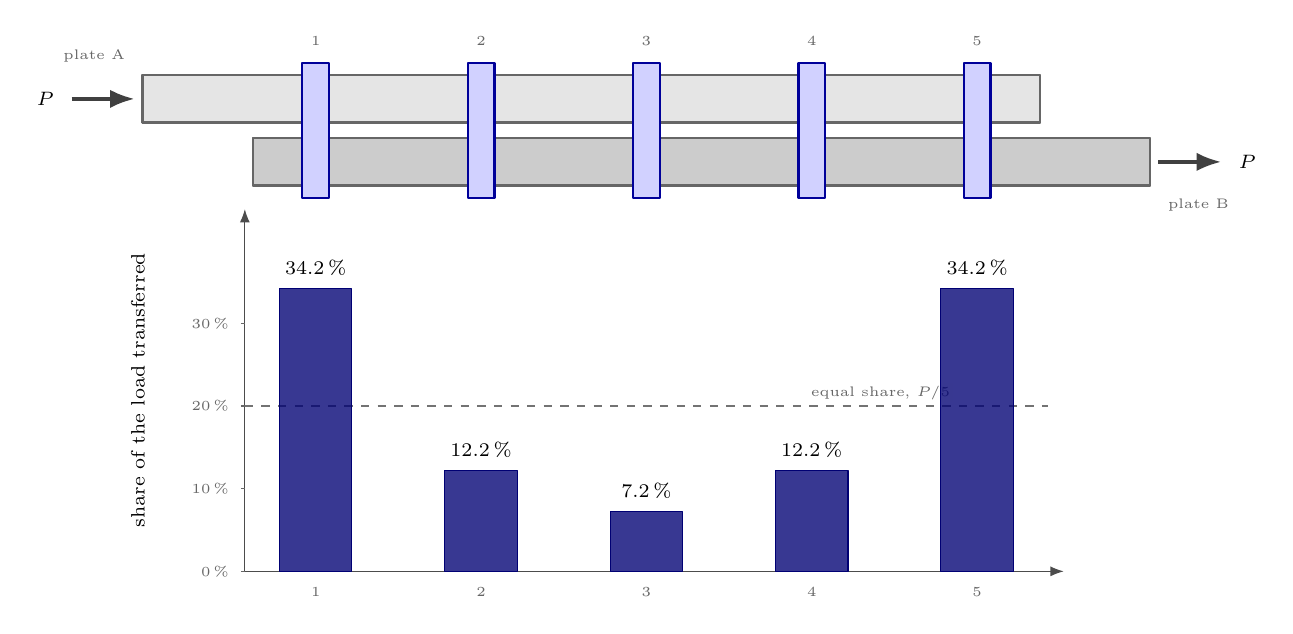
\begin{tikzpicture}[>=Latex,line join=round]
\tikzset{
  pa/.style={fill=black!10,draw=black!60,thick},
  pb/.style={fill=black!20,draw=black!60,thick},
  blt/.style={fill=blue!18,draw=blue!60!black,thick},
  ld/.style={->,black!75,line width=1.3pt},
  lb/.style={font=\scriptsize},
  sm/.style={font=\tiny,text=black!60}
}
\def\s{2.1}       % fastener spacing on the drawing

% ================= the splice =================
\begin{scope}[yshift=0cm]
\fill[pa] (-2.2,0.10) rectangle (9.2,0.70);
\draw[black!60,thick] (-2.2,0.10) rectangle (9.2,0.70);
\fill[pb] (-0.8,-0.70) rectangle (10.6,-0.10);
\draw[black!60,thick] (-0.8,-0.70) rectangle (10.6,-0.10);
\foreach \i in {0,1,2,3,4}{
  \pgfmathsetmacro\xx{\i*\s}
  \fill[blt] (\xx-0.17,-0.86) rectangle (\xx+0.17,0.86);
  \node[sm,anchor=south] at (\xx,0.95) {\the\numexpr\i+1\relax};
}
\draw[ld] (-3.1,0.40) -- (-2.3,0.40);
\node[lb,anchor=east] at (-3.2,0.40) {$P$};
\draw[ld] (10.7,-0.40) -- (11.5,-0.40);
\node[lb,anchor=west] at (11.6,-0.40) {$P$};
\node[sm,anchor=east] at (-2.3,0.95) {plate A};
\node[sm,anchor=west] at (10.7,-0.95) {plate B};
\end{scope}

% ================= the bar chart =================
\begin{scope}[yshift=-5.6cm]
\def\h{0.105}      % percent -> cm
\draw[->,black!70] (-0.9,0) -- (9.5,0);
\draw[->,black!70] (-0.9,0) -- (-0.9,4.6);
\node[lb,anchor=south,rotate=90] at (-2.05,2.3) {share of the load transferred};
\foreach \p in {0,10,20,30}{
  \draw[black!60] (-0.95,\p*\h) -- (-0.9,\p*\h);
  \node[sm,anchor=east] at (-0.98,\p*\h) {\p\,\%};}
% equal-share reference
\draw[dashed,black!55] (-0.9,20*\h) -- (9.3,20*\h);
\node[sm,anchor=west,fill=white,inner sep=1pt] at (6.25,20*\h+0.17) {equal share, $P/5$};
% bars
\foreach \i/\v in {0/34.2, 1/12.2, 2/7.2, 3/12.2, 4/34.2}{
  \pgfmathsetmacro\xx{\i*\s}
  \fill[blue!45!black,opacity=0.78] (\xx-0.46,0) rectangle (\xx+0.46,\v*\h);
  \draw[blue!45!black] (\xx-0.46,0) rectangle (\xx+0.46,\v*\h);
  \node[lb,anchor=south] at (\xx,\v*\h+0.04) {\v\,\%};
  \node[sm,anchor=north] at (\xx,-0.08) {\the\numexpr\i+1\relax};}
\end{scope}

\end{tikzpicture}
}
\vfill
\raggedright
\alert{That is wrong}, and knowing how wrong is the difference between a static check and a fatigue
check.
\end{frame}

\begin{frame}{Why the ends carry more}
At the \textbf{first} fastener, plate A still carries the whole load and plate B carries none. The
two plates strain very differently, so the slip across the joint --- and the fastener load --- is
greatest there.
\vspace{2pt}
By the middle, both plates carry similar loads, strain similarly, and the fasteners between them are
barely working.
\vfill
\begin{columns}[T]
\begin{column}{0.48\textwidth}
\begin{alertblock}{1. Rows of many fasteners are inefficient}
At five, the middle one takes \SI{7}{\percent}. At seven, \SI{2}{\percent}.
\vspace{2pt}
Beyond about four in a line, extra fasteners add holes, weight and cost --- and almost no strength.
\end{alertblock}
\end{column}
\begin{column}{0.48\textwidth}
\begin{alertblock}{2. The end fastener cracks first}
It is critical \textbf{twice}: highest bearing load \emph{and} highest bypass stress.
\vspace{2pt}
Which is exactly what the full-scale lap-splice testing in Lecture 5 found.
\end{alertblock}
\end{column}
\end{columns}
\end{frame}

\begin{frame}{Load transfer and bypass --- two stresses at one hole}
\begin{columns}[T]
\begin{column}{0.48\textwidth}
\begin{block}{Bearing}
from the load that fastener \textbf{transfers}
\end{block}
\end{column}
\begin{column}{0.48\textwidth}
\begin{block}{Bypass}
tension from the load that simply \textbf{passes by}, on its way to the next fastener
\end{block}
\end{column}
\end{columns}
\vfill
The end fastener has the highest transfer \emph{and} still has substantial bypass. It is the worst
combination in the joint.
\vfill
\begin{alertblock}{}
\centering
A static check that divides the load equally \textbf{will not find this}. Detailed joint analysis in
industry uses a load-transfer model, not a division.
\end{alertblock}
\end{frame}


\section{Rivets}

\begin{frame}{Why an aeroplane is still held together with rivets}
A rivet is a \textbf{shear joint}, so everything from the last two sections applies unchanged ---
four failure modes, edge distance, pitch, and the end fastener carrying the most.
\vfill
\begin{columns}[T]
\begin{column}{0.48\textwidth}
\begin{block}{What it gives you}
\begin{itemize}\footnotesize
\item \textbf{No preload to lose.} The entire first half of this lecture --- separation, relaxation,
  torque scatter --- simply does not apply.
\item Light, cheap, and installed in seconds, by the million.
\item The finished joint is \textbf{visible and measurable} from outside.
\end{itemize}
\end{block}
\end{column}
\begin{column}{0.48\textwidth}
\begin{alertblock}{What it costs you}
\begin{itemize}\footnotesize
\item \textbf{Permanent.} Removal means drilling it out, and that damages the hole.
\item No clamp force you can rely on --- so no friction, and the joint works in bearing.
\item One chance. A badly driven rivet is a repair, not an adjustment.
\end{itemize}
\end{alertblock}
\end{column}
\end{columns}
\end{frame}

\begin{frame}{Three families, all still in service}
\centering
\resizebox{0.99\textwidth}{!}{% Three fastener families still in aerospace use, each shown before and after installation.
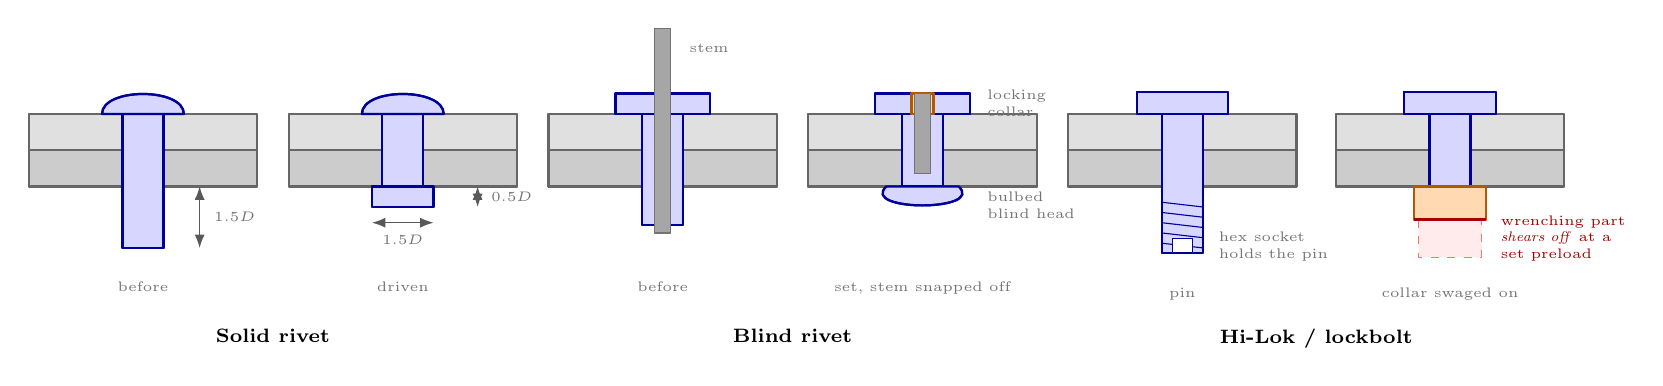
\begin{tikzpicture}[>=Latex,line join=round]
\tikzset{
  sh/.style={fill=black!12,draw=black!60,thick},
  sh2/.style={fill=black!20,draw=black!60,thick},
  riv/.style={fill=blue!16,draw=blue!60!black,thick},
  col/.style={fill=orange!30,draw=orange!70!black,thick},
  stem/.style={fill=black!35,draw=black!55,thin},
  gone/.style={fill=red!8,draw=red!55,thin,dashed},
  dimn/.style={<->,gray!70!black,thin},
  ar/.style={->,red!70!black,line width=1.1pt},
  ttl/.style={font=\scriptsize\bfseries,align=center,text width=5.0cm,anchor=north},
  sub/.style={font=\tiny,align=center,text width=5.2cm,text=black!60,anchor=north},
  st/.style={font=\tiny,text=black!55,align=center}
}
\def\D{0.52}          % rivet diameter on the drawing

% two sheets, centred on x
\newcommand{\sheets}[1]{%
  \fill[sh]  (#1-1.45,0) rectangle (#1+1.45,0.46);
  \fill[sh2] (#1-1.45,-0.46) rectangle (#1+1.45,0);
  \draw[black!60,thick] (#1-1.45,-0.46) rectangle (#1+1.45,0.46);
  \draw[black!60] (#1-1.45,0) -- (#1+1.45,0);}

%================= 1. solid rivet =================
\begin{scope}[yshift=0cm]
% -- before --
\def\x{0}
\sheets{\x}
\fill[white] (\x-\D/2,-0.46) rectangle (\x+\D/2,0.46);
\fill[riv] (\x-\D/2,-1.24) rectangle (\x+\D/2,0.46);
\fill[riv] (\x-0.52,0.46) .. controls (\x-0.52,0.80) and (\x+0.52,0.80) .. (\x+0.52,0.46) -- cycle;
\draw[blue!60!black,thick] (\x-0.52,0.46) .. controls (\x-0.52,0.80) and (\x+0.52,0.80) .. (\x+0.52,0.46);
\draw[blue!60!black,thick] (\x-\D/2,0.46) -- (\x-\D/2,-1.24) -- (\x+\D/2,-1.24) -- (\x+\D/2,0.46);
\draw[dimn] (\x+0.72,-0.46) -- (\x+0.72,-1.24);
\node[st,anchor=west] at (\x+0.78,-0.85) {$1.5D$};
\node[st,anchor=north] at (\x,-1.55) {before};
% -- after --
\def\x{3.3}
\sheets{\x}
\fill[white] (\x-\D/2,-0.46) rectangle (\x+\D/2,0.46);
\fill[riv] (\x-\D/2,-0.46) rectangle (\x+\D/2,0.46);
\fill[riv] (\x-0.52,0.46) .. controls (\x-0.52,0.80) and (\x+0.52,0.80) .. (\x+0.52,0.46) -- cycle;
\draw[blue!60!black,thick] (\x-0.52,0.46) .. controls (\x-0.52,0.80) and (\x+0.52,0.80) .. (\x+0.52,0.46);
% the shop head: 1.5D wide, 0.5D high
\fill[riv] (\x-0.75*\D,-0.46) rectangle (\x+0.75*\D,-0.46-0.5*\D);
\draw[blue!60!black,thick] (\x-0.75*\D,-0.46) rectangle (\x+0.75*\D,-0.46-0.5*\D);
\draw[blue!60!black,thick] (\x-\D/2,0.46) -- (\x-\D/2,-0.46) (\x+\D/2,0.46) -- (\x+\D/2,-0.46);
\draw[dimn] (\x-0.75*\D,-0.92) -- (\x+0.75*\D,-0.92);
\node[st,anchor=north] at (\x,-0.95) {$1.5D$};
\draw[dimn] (\x+0.95,-0.46) -- (\x+0.95,-0.46-0.5*\D);
\node[st,anchor=west] at (\x+1.00,-0.59) {$0.5D$};
\node[st,anchor=north] at (\x,-1.55) {driven};
\node[ttl] at (1.65,-2.15) {Solid rivet};
\end{scope}

%================= 2. blind rivet =================
\begin{scope}[xshift=6.6cm]
% -- before --
\def\x{0}
\sheets{\x}
\fill[white] (\x-\D/2,-0.46) rectangle (\x+\D/2,0.46);
\fill[riv] (\x-\D/2,-0.95) rectangle (\x+\D/2,0.46);
\fill[riv] (\x-0.60,0.46) rectangle (\x+0.60,0.72);
\draw[blue!60!black,thick] (\x-0.60,0.46) rectangle (\x+0.60,0.72);
\draw[blue!60!black,thick] (\x-\D/2,0.46) -- (\x-\D/2,-0.95) -- (\x+\D/2,-0.95) -- (\x+\D/2,0.46);
\fill[stem] (\x-0.10,-1.05) rectangle (\x+0.10,1.55);
\node[st,anchor=west] at (\x+0.22,1.30) {stem};
\node[st,anchor=north] at (\x,-1.55) {before};
% -- after --
\def\x{3.3}
\sheets{\x}
\fill[white] (\x-\D/2,-0.46) rectangle (\x+\D/2,0.46);
\fill[riv] (\x-\D/2,-0.46) rectangle (\x+\D/2,0.46);
\fill[riv] (\x-0.60,0.46) rectangle (\x+0.60,0.72);
\draw[blue!60!black,thick] (\x-0.60,0.46) rectangle (\x+0.60,0.72);
% bulbed blind head
\fill[riv] (\x-0.46,-0.46) .. controls (\x-0.80,-0.78) and (\x+0.80,-0.78) .. (\x+0.46,-0.46) -- cycle;
\draw[blue!60!black,thick] (\x-0.46,-0.46) .. controls (\x-0.80,-0.78) and (\x+0.80,-0.78) .. (\x+0.46,-0.46);
\draw[blue!60!black,thick] (\x-\D/2,0.46) -- (\x-\D/2,-0.46) (\x+\D/2,0.46) -- (\x+\D/2,-0.46);
\fill[col] (\x-0.14,0.46) rectangle (\x+0.14,0.72);
\draw[orange!70!black,thick] (\x-0.14,0.46) rectangle (\x+0.14,0.72);
\fill[stem] (\x-0.10,-0.30) rectangle (\x+0.10,0.72);
\node[st,anchor=west,align=left] at (\x+0.70,0.60) {locking\\ collar};
\node[st,anchor=west,align=left] at (\x+0.70,-0.70) {bulbed\\ blind head};
\node[st,anchor=north] at (\x,-1.55) {set, stem snapped off};
\node[ttl] at (1.65,-2.15) {Blind rivet};
\end{scope}

%================= 3. Hi-Lok =================
\begin{scope}[xshift=13.2cm]
% -- before --
\def\x{0}
\sheets{\x}
\fill[white] (\x-\D/2,-0.46) rectangle (\x+\D/2,0.46);
\fill[riv] (\x-\D/2,-1.30) rectangle (\x+\D/2,0.46);
\fill[riv] (\x-0.58,0.46) rectangle (\x+0.58,0.74);
\draw[blue!60!black,thick] (\x-0.58,0.46) rectangle (\x+0.58,0.74);
\draw[blue!60!black,thick] (\x-\D/2,0.46) -- (\x-\D/2,-1.30) -- (\x+\D/2,-1.30) -- (\x+\D/2,0.46);
\foreach \k in {0,1,...,4}{\draw[blue!60!black,thin] (\x-\D/2,-0.66-0.13*\k) -- (\x+\D/2,-0.72-0.13*\k);}
\fill[white,draw=blue!60!black,thin] (\x-0.13,-1.30) rectangle (\x+0.13,-1.12);
\node[st,anchor=west,align=left] at (\x+0.34,-1.22) {hex socket\\ holds the pin};
\node[st,anchor=north] at (\x,-1.62) {pin};
% -- after --
\def\x{3.4}
\sheets{\x}
\fill[white] (\x-\D/2,-0.46) rectangle (\x+\D/2,0.46);
\fill[riv] (\x-\D/2,-0.92) rectangle (\x+\D/2,0.46);
\fill[riv] (\x-0.58,0.46) rectangle (\x+0.58,0.74);
\draw[blue!60!black,thick] (\x-0.58,0.46) rectangle (\x+0.58,0.74);
\draw[blue!60!black,thick] (\x-\D/2,0.46) -- (\x-\D/2,-0.92) -- (\x+\D/2,-0.92) -- (\x+\D/2,0.46);
\fill[col] (\x-0.46,-0.46) rectangle (\x+0.46,-0.88);
\draw[orange!70!black,thick] (\x-0.46,-0.46) rectangle (\x+0.46,-0.88);
% the wrenching portion that has broken away
\fill[gone] (\x-0.40,-0.88) rectangle (\x+0.40,-1.36);
\draw[red!65!black,line width=1.1pt] (\x-0.46,-0.88) -- (\x+0.46,-0.88);
\node[st,anchor=west,align=left,text=red!65!black] at (\x+0.52,-1.12)
  {wrenching part\\ \emph{shears off} at a\\ set preload};
\node[st,anchor=north] at (\x,-1.62) {collar swaged on};
\node[ttl] at (1.70,-2.15) {Hi-Lok / lockbolt};
\end{scope}

\end{tikzpicture}
}
\vfill
\raggedright
\footnotesize
\textbf{Solid} where you can reach both sides. \textbf{Blind} where you cannot. \textbf{Pin-and-collar}
where you want bolt strength with rivet installation speed --- which on a modern airframe is most of
the primary structure.
\end{frame}

\begin{frame}{The solid rivet, and how to read one}
\centering\footnotesize
\begin{tabular}{@{}llll@{}}
\toprule
Alloy & Code & Head marking & Part number\\
\midrule
1100-F & A & plain & MS20470A \ / \ MS20426A\\
\textbf{2117-T4} & \textbf{AD} & \textbf{dimple} & MS20470AD \ / \ MS20426AD\\
5056-H32 & B & raised cross & MS20470B \ / \ MS20426B\\
2017-T4 & D & raised dot & MS20470D \ / \ MS20426D\\
2024-T4 & DD & raised double dash & MS20470DD \ / \ MS20426DD\\
7050-T73 & E & indented ring & MS20470E \ / \ MS20426E\\
Ti 45Cb & T & indented diamond & MS20470T \ / \ MS20426T\\
\bottomrule
\end{tabular}
\vfill
\raggedright
\textbf{MS20470} is the universal head; \textbf{MS20426} is the $100^\circ$ countersunk head ---
the same $100^\circ$ as Lecture 5, and the same knife-edge rule applies.
\vfill
\centering
\alert{The alloy is stamped on the head.} You can identify a rivet in an airframe without paperwork.
\end{frame}

\begin{frame}{Ice-box rivets --- the alloy that fights back}
The strong aluminium rivet alloys are \textbf{heat treatable}, which means they \alert{age-harden at
room temperature} --- within minutes of coming out of the freezer.
\vfill
\centering\small
\begin{tabular}{@{}lll@{}}
\toprule
Alloy & Stored & Working time at room temperature\\
\midrule
2017-T (D) & below \SI{32}{\degree F}, up to 2 weeks & about \textbf{1 hour}\\
2024-T (DD) & below \SI{32}{\degree F}, up to 2 weeks & about \textbf{10 minutes}\\
\bottomrule
\end{tabular}
\vfill
\raggedright
Past that, the rivet is too hard to drive without cracking, and it must go back for
re-heat-treatment.
\vfill
\begin{alertblock}{Which is exactly why 2117-T4 (AD) dominates}
It is driven \textbf{as received} --- no refrigeration, no clock, no re-heat-treatment. A slightly
weaker rivet that can always be installed correctly beats a stronger one that often is not.
\end{alertblock}
\end{frame}

\begin{frame}{Driving: the shop head \emph{is} the inspection}
\begin{columns}[T]
\begin{column}{0.46\textwidth}
\begin{block}{The three numbers}
\begin{itemize}\footnotesize
\item Protrude \textbf{1.5\,$D$} through the joint before driving.
\item Finished shop head: \textbf{1.5\,$D$} across, at least \textbf{0.5\,$D$} high.
\item Keep $D \le 5.5\,t$ of the \emph{thinnest} sheet, or the material distorts.
\end{itemize}
\end{block}
\end{column}
\begin{column}{0.50\textwidth}
\begin{alertblock}{Why this matters more than it looks}
A bolt's preload is invisible once installed --- $\pm\SI{25}{\percent}$ and no way to check.
\vspace{3pt}
A rivet's quality is a \textbf{dimension}. Too short and the head is undersized; too long and the
shank bends over instead of swelling.
\vspace{3pt}
\alert{You can put a gauge on it.}
\end{alertblock}
\end{column}
\end{columns}
\end{frame}

\begin{frame}{Blind fasteners --- when you can only reach one side}
\textbf{CherryMAX} and similar: a sleeve, a stem, and a \textbf{mechanical} locking collar. The stem
pulls, bulbs the blind head, then snaps off flush.
\vfill
\begin{columns}[T]
\begin{column}{0.46\textwidth}
\begin{block}{Why mechanical lock}
A friction-locked stem can shake out under vibration. The visible locking collar is what makes it
structural --- and inspectable.
\end{block}
\end{column}
\begin{column}{0.50\textwidth}
\begin{alertblock}{Where they may not go}
Fluid-tight areas \ $\cdot$ \ engine air intakes \ $\cdot$ \ control surfaces \ $\cdot$ \ hinges \
$\cdot$ \ landing gear fittings.
\vspace{2pt}
{\footnotesize And on a metal airframe repair, only where the manufacturer or the authority has
specifically approved them.}
\end{alertblock}
\end{column}
\end{columns}
\vfill
\centering
The honest rule: \alert{blind rivets are not used where a driven rivet can be installed.}
\end{frame}

\begin{frame}{Hi-Lok and lockbolts --- the answer to Lecture 5's problem}
A two-piece pin and collar. The pin is held by a \textbf{hex socket in its own end}; the collar is
torqued until its wrenching portion \alert{shears off at a built-in fracture groove}.
\vfill
\begin{alertblock}{That shear-off happens at a predetermined preload}
So the fastener \textbf{cannot be overtorqued}, and \textbf{no torque check is needed}.
\vspace{3pt}
Recall \S11.3 of Lecture 5: a torque wrench delivers the intended preload to $\pm\SI{25}{\percent}$.
Hi-Lok does not measure the preload better --- \textbf{it removes the measurement from the problem}.
\end{alertblock}
\vfill
\footnotesize
Interference fit in aluminium (not exceeding \SI{0.002}{in}); \textbf{clearance} fit in steel,
titanium and composites. \ Hi-Tigue adds a bead that cold-works the hole; Hi-Lite is the lighter
titanium version, with lower clamp-up --- and its collars are \emph{not} interchangeable.
\end{frame}

\begin{frame}{Where rivets stop}
\begin{alertblock}{Composites}
\textbf{Solid rivets must not be used in composite structure.} Driving one expands the shank into an
interference fit, which overstresses the hole and \textbf{delaminates the laminate}.
\vspace{3pt}
What is good practice in aluminium --- an interference fit to improve fatigue life --- is damage in a
laminate. Composites get clearance-fit pin-and-collar fasteners in titanium or A286.
\end{alertblock}
\vfill
\begin{columns}[T]
\begin{column}{0.48\textwidth}
\begin{block}{And increasingly}
bonding, co-cured structure, and friction stir welding remove the hole altogether --- and with it the
stress concentration, the sealing problem and the leak path.
\end{block}
\end{column}
\begin{column}{0.48\textwidth}
\begin{block}{But}
a bonded joint cannot be inspected the way a rivet line can, and it cannot be taken apart. The rivet
survives because it is \textbf{visible}.
\end{block}
\end{column}
\end{columns}
\end{frame}

\section{Eccentric bolt groups}

\begin{frame}{When the load misses the centroid}
\centering
\resizebox{!}{5.8cm}{% Eccentric shear on a bolt group. Numbers are Example 6.3: P = 18 kN at e = 250 mm,
% six bolts at (+-40, 0/+-60) mm, sum r^2 = 24 000 mm^2.
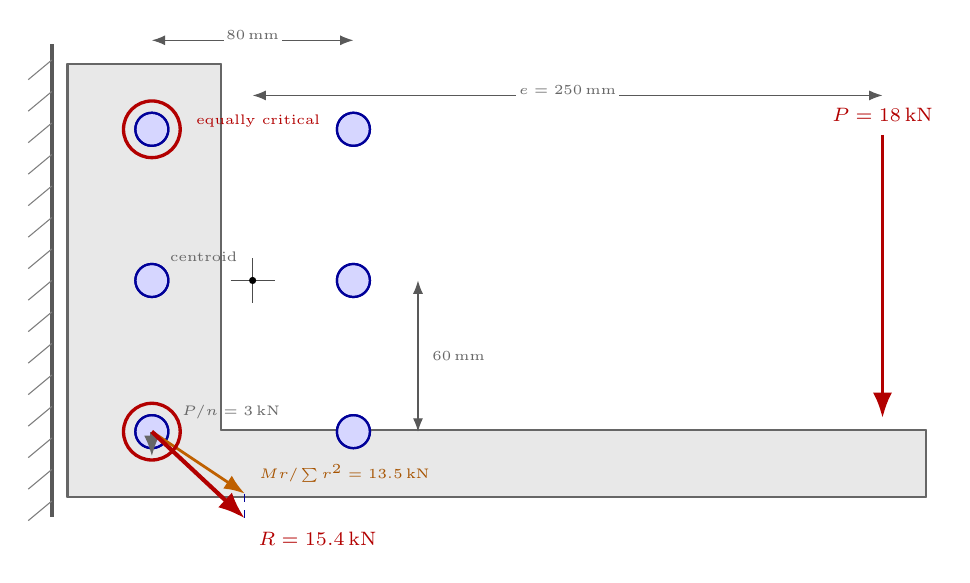
\begin{tikzpicture}[>=Latex,line join=round]
\tikzset{
  brk/.style={fill=black!9,draw=black!60,thick},
  blt/.style={fill=blue!16,draw=blue!60!black,thick},
  ld/.style={->,red!70!black,line width=1.4pt},
  vd/.style={->,black!60,line width=1.0pt},
  vm/.style={->,orange!75!black,line width=1.0pt},
  vr/.style={->,red!70!black,line width=1.5pt},
  lb/.style={font=\scriptsize},
  sm/.style={font=\tiny,text=black!60},
  dimn/.style={<->,gray!70!black,thin}
}
\def\g{0.032}    % mm -> cm
\def\f{0.105}    % kN -> cm

% ---- bracket ----
\fill[brk] (-2.35,-2.75) -- (8.55,-2.75) -- (8.55,-1.9) -- (-0.4,-1.9)
        -- (-0.4,2.75) -- (-2.35,2.75) -- cycle;
\draw[black!60,thick] (-2.35,-2.75) -- (8.55,-2.75) -- (8.55,-1.9) -- (-0.4,-1.9)
        -- (-0.4,2.75) -- (-2.35,2.75) -- cycle;
% wall
\draw[black!65,line width=1.2pt] (-2.55,-3.0) -- (-2.55,3.0);
\foreach \k in {-2.8,-2.4,...,2.9}{\draw[black!50,thin] (-2.55,\k) -- (-2.85,\k-0.25);}

% ---- bolts ----
\foreach \X/\Y in {-40/-60, 40/-60, -40/0, 40/0, -40/60, 40/60}{
  \pgfmathsetmacro\xx{\X*\g}\pgfmathsetmacro\yy{\Y*\g}
  \fill[blt] (\xx,\yy) circle (0.21);
  \draw[blue!60!black,thick] (\xx,\yy) circle (0.21);}

% ---- centroid ----
\draw[black!70,thin] (-0.28,0) -- (0.28,0) (0,-0.28) -- (0,0.28);
\fill[black] (0,0) circle (1.3pt);
\node[sm,anchor=south east] at (-0.07,0.12) {centroid};

% ---- geometry dimensions ----
\draw[dimn] (-40*\g,3.05) -- (40*\g,3.05);
\node[sm,anchor=south,fill=white,inner sep=1pt] at (0,3.02) {\SI{80}{mm}};
\draw[dimn] (2.1,-60*\g) -- (2.1,0);
\node[sm,anchor=west] at (2.16,-0.96) {\SI{60}{mm}};

% ---- applied load ----
\draw[ld] (250*\g,1.85) -- (250*\g,-1.75);
\node[lb,text=red!70!black,anchor=south] at (250*\g,1.90) {$P=\SI{18}{kN}$};
\draw[dimn] (0,2.35) -- (250*\g,2.35);
\node[sm,anchor=south,fill=white,inner sep=1pt] at (4.0,2.32) {$e=\SI{250}{mm}$};

% ---- the two critical bolts, with the vector sum drawn on the lower one ----
\pgfmathsetmacro\cx{-40*\g}\pgfmathsetmacro\cy{-60*\g}
\draw[vd] (\cx,\cy) -- (\cx,{\cy-3.0*\f});
\node[sm,anchor=south west] at (\cx+0.26,{\cy+0.04}) {$P/n=\SI{3}{kN}$};
\draw[vm] (\cx,\cy) -- ({\cx+11.25*\f},{\cy-7.5*\f});
\node[sm,text=orange!65!black,anchor=south west] at ({\cx+11.25*\f+0.06},{\cy-7.5*\f+0.02})
  {$Mr/\sum r^2 = \SI{13.5}{kN}$};
\draw[vr] (\cx,\cy) -- ({\cx+11.25*\f},{\cy-10.5*\f});
\node[font=\scriptsize\bfseries,text=red!70!black,anchor=north west] at ({\cx+11.25*\f+0.05},{\cy-10.5*\f-0.05})
  {$R=\SI{15.4}{kN}$};
\draw[blue!60!black,dashed] ({\cx+11.25*\f},{\cy-7.5*\f}) -- ({\cx+11.25*\f},{\cy-10.5*\f});
\draw[red!70!black,very thick] (\cx,\cy) circle (0.36);
\draw[red!70!black,very thick] (\cx,{-\cy}) circle (0.36);
\node[sm,text=red!70!black,anchor=west] at (\cx+0.44,{-\cy+0.10}) {equally critical};

\end{tikzpicture}
}
\end{frame}

\begin{frame}{The method, in four steps}
\begin{enumerate}
\item \textbf{Find the centroid.} For identical fasteners, the average of their coordinates.
\item \textbf{Direct shear}, identical on every fastener: \quad $F_d = P/n$
\item \textbf{Moment shear}, perpendicular to the radius and proportional to it:
  \[ M = P\,e, \qquad F_i = \frac{M\,r_i}{\sum_j r_j^{2}} \]
\item \textbf{Add as vectors} and take the largest resultant.
\end{enumerate}
\vfill
\begin{alertblock}{}
\centering
The critical fastener is \alert{not} always the one furthest from the centroid --- it is the one
where the two components \textbf{align best}.
\end{alertblock}
\end{frame}

\begin{frame}{Example 6.3 --- a bracket with six bolts}
Six bolts at $(\pm40,0)$ and $(\pm40,\pm60)$ mm. $P=\SI{18}{kN}$ acting \SI{250}{mm} from the
centroid. \ $\sum r^2 = \SI{24000}{mm^2}$, \ $M=\SI{4500}{kN.mm}$.
\vfill
\centering\small
\begin{tabular}{@{}lccc@{}}
\toprule
Bolt (mm) & $r$ (mm) & $F_M$ (kN) & $R$ (kN)\\
\midrule
$(-40,-60)$ & 72.1 & 13.5 & $\mathbf{15.4}$\\
$(-40,+60)$ & 72.1 & 13.5 & $\mathbf{15.4}$\\
$(+40,\pm60)$ & 72.1 & 13.5 & 12.1\\
$(-40,0)$ & 40.0 & 7.5 & 10.5\\
$(+40,0)$ & 40.0 & 7.5 & 4.5\\
\bottomrule
\end{tabular}
\vfill
\raggedright
Moment term \SI{13.5}{kN} against \SI{3}{kN} of direct shear --- a ratio of \textbf{four and a
half}.
\end{frame}

\begin{frame}{What that ratio tells you to do}
\begin{center}\Large
In an eccentric joint, the \alert{moment almost always dominates}.
\end{center}
\vfill
\begin{alertblock}{So the most effective design change is not a bigger bolt}
It is \textbf{spreading the pattern} --- because $\sum r^2$ grows with the \emph{square} of the
spacing.
\vspace{3pt}
Double the spacing and the moment force on each bolt roughly halves.
\end{alertblock}
\vfill
\centering
Two bolts were equally critical here. In a real bracket, manufacturing scatter decides which one
goes first --- so you check both.
\end{frame}

\section{Combined loading, and the grip}

\begin{frame}{Combined tension and shear}
\[
R_s=\frac{\text{applied shear}}{\text{shear allowable}},
\qquad
R_t=\frac{\text{applied tension}}{\text{tension allowable}}
\]
\vfill
\begin{columns}[T]
\begin{column}{0.48\textwidth}
\begin{block}{Shear plane in the \emph{shank}}
\[ R_s^{3}+R_t^{2}=1 \]
{\footnotesize shear allowable on the body, tension allowable on the threads. Used since the
AN-series bolts.}
\end{block}
\end{column}
\begin{column}{0.48\textwidth}
\begin{block}{Shear plane in the \emph{thread}}
\[ R_s^{2}+R_t^{2}=1 \]
{\footnotesize the commonly assumed form.}
\end{block}
\end{column}
\end{columns}
\vfill
\begin{alertblock}{Read those together}
At $R_s=0.5$ the cubic leaves $R_t=0.93$; the square leaves $R_t=0.87$. \textbf{The grip length
decides which equation you are entitled to use.}
\end{alertblock}
\end{frame}

\begin{frame}{A caution worth carrying}
\begin{alertblock}{The interaction equation is an empirical curve fit}
NASA testing has found $R_s^3+R_t^2=1$ can \textbf{overpredict} measured combined strength by up to
\SI{7}{\percent} when \emph{actual} strengths are used as allowables.
\vspace{3pt}
It is conservative when \textbf{minimum specified} strengths are used --- which is how you will
always use it.
\end{alertblock}
\vfill
The same work notes that using this form with both allowables taken from the \emph{same}
cross-section is not recommended.
\vfill
\centering
\alert{Know what your allowables are before you trust the exponent.}
\end{frame}

\begin{frame}{What the grip length decides}
\begin{enumerate}
\item \textbf{Which area resists the shear.} Shank $\pi D^2/4$, or thread $A_t$. For an M10 that is
  \SI{78.5}{mm^2} against \SI{58.0}{mm^2} --- a \SI{26}{\percent} loss before any other effect.
\item \textbf{Whether the bearing surface is a notch.} The thread root sits exactly where the
  bearing pressure peaks --- and it damages the hole.
\item \textbf{Which interaction equation you may use.} $R_s^3$ or $R_s^2$.
\item \textbf{Whether the head seats at all.} Too long, and it bottoms on the run-out instead of the
  member --- so no preload is ever developed.
\end{enumerate}
\vfill
\begin{alertblock}{}
\centering
The grip is a \textbf{dimension on the drawing}, derived from the stack and checked against the
shear plane. It is not something the shop floor picks out of a bin.
\end{alertblock}
\end{frame}

\begin{frame}{Three more things that belong to joints, not fasteners}
\begin{alertblock}{Never mix fastener types in one load path}
Bolts and rivets in the same joint do not share: the \textbf{stiffer one takes the load until it
fails}. Same for a close-tolerance fastener beside a clearance one.
\end{alertblock}
\begin{alertblock}{A shim is a load path}
A shimmed joint transmits load through the shim. Liquid or tapered shims change the fastener bending
and the effective grip. \textbf{Shims are specified, not improvised.}
\end{alertblock}
\begin{alertblock}{Single-lap joints bend}
The load path is offset by the sheet thickness, so the splice carries a \textbf{secondary bending
moment}. It is why a single-lap joint has a shorter fatigue life than its static margin suggests ---
and why doublers are symmetric wherever weight allows.
\end{alertblock}
\end{frame}

\section{What to take away}

\begin{frame}{What to take away}
\begin{columns}[T]
\begin{column}{0.48\textwidth}
\begin{block}{Tension joints}
\begin{itemize}\footnotesize
\item The preload \textbf{is} the design.
\item Check yield, separation, fatigue. Fatigue usually governs.
\item \alert{Reduce $C$ to improve fatigue, not $F_i$.}
\item Separation is a cliff, not a limit.
\end{itemize}
\end{block}
\end{column}
\begin{column}{0.48\textwidth}
\begin{block}{Shear joints}
\begin{itemize}\footnotesize
\item Check all four modes.
\item Thin sheet: the plate governs.
\item Edge distance guards shear-out; pitch guards net tension.
\item \alert{Add rows, not fasteners in a line.}
\item Design the \textbf{end} fastener for fatigue.
\end{itemize}
\end{block}
\end{column}
\end{columns}
\vfill
\centering
\large And specify the grip --- it decides the area, the notch, the equation, and whether the head
seats at all.
\end{frame}

\end{document}
